%%%%%%%%%%%%%%%%%%%%%%%%%%%%%%%%%%%%%%%%%
% Beamer Presentation
% LaTeX Template
% Version 1.0 (10/11/12)
%
% This template has been downloaded from:
% http://www.LaTeXTemplates.com
%
% License:
% CC BY-NC-SA 3.0 (http://creativecommons.org/licenses/by-nc-sa/3.0/)
%
%%%%%%%%%%%%%%%%%%%%%%%%%%%%%%%%%%%%%%%%%

%----------------------------------------------------------------------------------------
%	PACKAGES AND THEMES
%----------------------------------------------------------------------------------------

\documentclass{beamer}
\usepackage[spanish]{babel}
\usepackage{amsthm}
\usepackage{bbding}
\usepackage[utf8]{inputenc}
%\usepackage{enumitem}

\mode<presentation> {

% The Beamer class comes with a number of default slide themes
% which change the colors and layouts of slides. Below this is a list
% of all the themes, uncomment each in turn to see what they look like.

%\usetheme{default}
%\usetheme{AnnArbor}
%\usetheme{Antibes}
%\usetheme{Bergen}
%\usetheme{Berkeley}
%\usetheme{Berlin}
%\usetheme{Boadilla}
%\usetheme{CambridgeUS}
%\usetheme{Copenhagen}
%\usetheme{Darmstadt}
%\usetheme{Dresden}
%\usetheme{Frankfurt}
%\usetheme{Goettingen}
%\usetheme{Hannover}
%\usetheme{Ilmenau}
%\usetheme{JuanLesPins}
%\usetheme{Luebeck}
\usetheme{Madrid}
%\usetheme{Malmoe}
%\usetheme{Marburg}
%\usetheme{Montpellier}
%\usetheme{PaloAlto}
%\usetheme{Pittsburgh}
%\usetheme{Rochester}
%\usetheme{Singapore}
%\usetheme{Szeged}
%\usetheme{Warsaw}

% As well as themes, the Beamer class has a number of color themes
% for any slide theme. Uncomment each of these in turn to see how it
% changes the colors of your current slide theme.

%\usecolortheme{albatross}
%\usecolortheme{beaver}
%\usecolortheme{beetle}
%\usecolortheme{crane}
%\usecolortheme{dolphin}
%\usecolortheme{dove}
%\usecolortheme{fly}
%\usecolortheme{lily}
%\usecolortheme{orchid}
%\usecolortheme{rose}
%\usecolortheme{seagull}
%\usecolortheme{seahorse}
%\usecolortheme{whale}
%\usecolortheme{wolverine}

%\setbeamertemplate{footline} % To remove the footer line in all slides uncomment this line
%\setbeamertemplate{footline}[page number] % To replace the footer line in all slides with a simple slide count uncomment this line

%\setbeamertemplate{navigation symbols}{} % To remove the navigation symbols from the bottom of all slides uncomment this line
}
\usepackage{color}
\usepackage{graphicx} % Allows including images
\usepackage{booktabs} % Allows the use of \toprule, \midrule and \bottomrule in tables
\setbeamertemplate{blocks}[rounded][shadow=true]
%----------------------------------------------------------------------------------------
%	TITLE PAGE
%----------------------------------------------------------------------------------------

\title[Presentación del TP2]{Semántica Web} % The short title appears at the bottom of every slide, the full title is only on the title page

\author{Federico Allocati, Sabrina Izcovich, Santiago Pernigotti, Germán Romano} % Your name
\institute[] % Your institution as it will appear on the bottom of every slide, may be shorthand to save space
{
Departamento de Computación\\ % Your institution for the title page
\medskip
%\textit{john@smith.com} % Your email address
}
\date{Viernes 20 de junio de 2015} % Date, can be changed to a custom date

\begin{document}

\begin{frame}
\titlepage % Print the title page as the first slide
\end{frame}

\begin{frame}
\frametitle{Contenidos} % Table of contents slide, comment this block out to remove it
\tableofcontents % Throughout your presentation, if you choose to use \section{} and \subsection{} commands, these will automatically be printed on this slide as an overview of your presentation
\end{frame}

%----------------------------------------------------------------------------------------
%	PRESENTATION SLIDES
%----------------------------------------------------------------------------------------

%------------------------------------------------
\section{Introducción} 
%------------------------------------------------
\begin{frame}
\frametitle{Material Analizado}
\begin{itemize}
\item \textbf{Optimizing Reformulated RDF Queries}, Damián A. Bursztyn, 2013

\end{itemize}
\end{frame}

%------------------------------------------------
\section{Contextualizando...} 
%------------------------------------------------
\subsection{Web Semántica}
\begin{frame}
\frametitle{¿Qué es la Web Semántica?} 
\begin{block}{Web Semántica}
\begin{itemize}
\item<1-> Web Extendida enfocada en el significado de las búsquedas.
\item<2-> Se procesa la información en términos de su semántica a través de operaciones bien definidas.
\item<3-> El software es capaz de procesar el contenido, razonar con este, combinarlo y realizar deducciones lógicas para resolver problemas cotidianos automáticamente.
\item<4-> Utiliza una infraestructura común mediante la cual es posible compartir, procesar y transferir información de forma sencilla.
\item<5-> Otorga una solución a problemas habituales en la búsqueda de información ocasionados por la sobrecarga de información y heterogeneidad de fuentes de información.
\end{itemize}
\end{block}
\end{frame}
%------------------------------------------------
\begin{frame}
\frametitle{Ejemplo} 
\begin{figure}[H] %[h] Aqui [b] para button [t] para top
\begin{center}
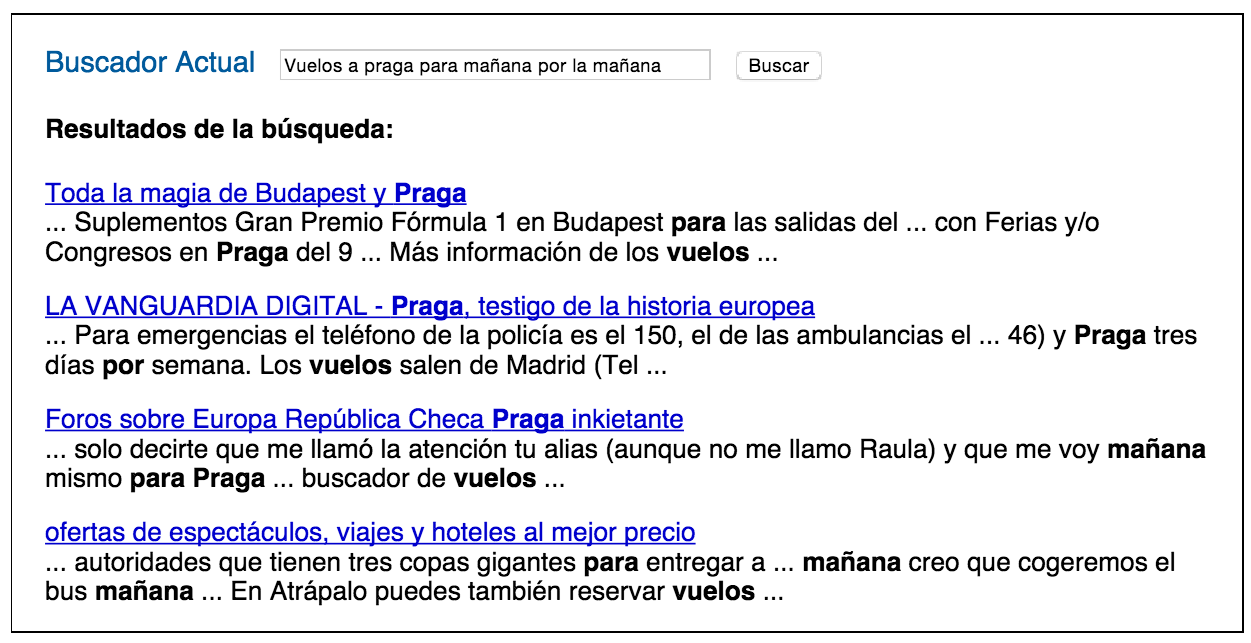
\includegraphics[width=340pt]{imgs/resultadoNormal}
\caption{Resultados obtenidos con un buscador normal.}
\end{center}
\end{figure}
\end{frame}
%------------------------------------------------
\begin{frame}
\frametitle{Ejemplo} 
\begin{figure}[H] %[h] Aqui [b] para button [t] para top
\begin{center}
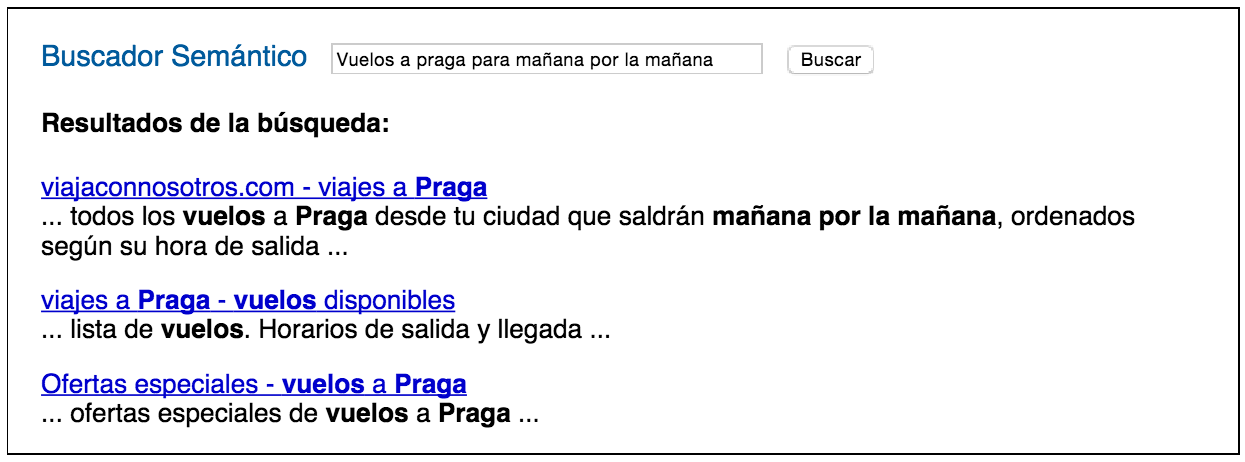
\includegraphics[width=340pt]{imgs/resultadoSemantico}
\caption{Resultados obtenidos con un buscador semántico.}
\end{center}
\end{figure}
\end{frame}
%------------------------------------------------
\subsection{RDF}
\begin{frame}[fragile] % Need to use the fragile option when verbatim is used in the slide
\frametitle{¿Qué es RDF?}
\begin{block}{Resource Description Framework}
\begin{itemize}
\item<1-> Modelo estándar para intercambio de datos en la Web.
\item<2-> En particular, es el formato de datos de la web semántica.
\item<3-> Tiene características que facilitan la fusión de datos a pesar de que sus esquemas de organización difieran.
\item<4-> Extiende la unión de estructuras en la Web nombrando las relaciones entre cosas.
\item<5-> La estructura de \textit{linking} forma un grafo dirigido y etiquetado donde los ejes representan la relación entre dos fuentes (los nodos).
\item<5-> Su utilización permite estructurar los datos a ser fusionados, expuestos y compartidos a través de diferentes aplicaciones.
\end{itemize}
\end{block}
\end{frame}

%------------------------------------------------
\begin{frame}[fragile]
\frametitle{Ejemplo}
\textit{``Javier Perez es el autor del documento cuya URL es http://www.dc.uba.ar/examen.pdf. Su mail es jperez@dc.uba.ar y su teléfono +54(11)4563-4567.''}
\begin{verbatim}
<?namespace href="http://dc.uba.ar/info-bibliografia" as="bib"?> 
<RDF:serialization> 
  <RDF:assertions href="http://dc.uba.ar/examen.pdf"> 
    <bib:autor> 
      <RDF:resource> 
        <bib:nombre>Javier Perez</bib:nombre> 
        <bib:mail>jperez@dc.uba.ar</bib:mail> 
        <bib:telefono>+54(11)4563-4567</bib:telefono> 
      </RDF:resource> 
    </bib:autor> 
  </RDF:assertions> 
</RDF:serialization>

\end{verbatim}
\end{frame}

%------------------------------------------------
\begin{frame}[fragile]
\frametitle{Ejemplo} 
\begin{center}
\begin{figure}[H] %[h] Aqui [b] para button [t] para top
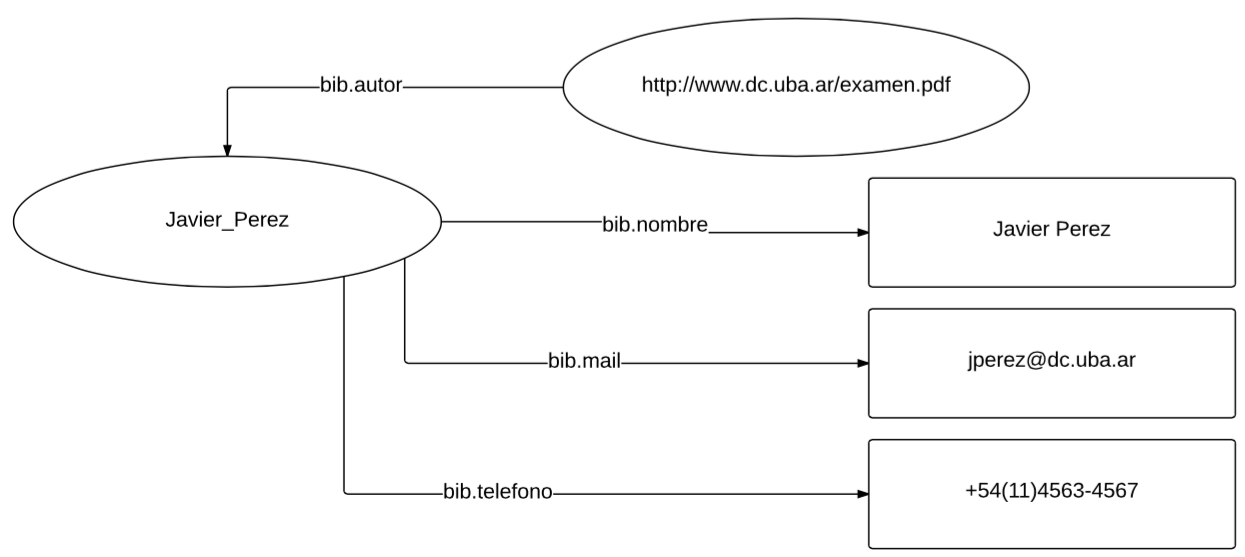
\includegraphics[width=300pt]{imgs/rdfModel}
\caption{Modelo RDF.}
\end{figure}
Los nodos son las elipses, los ejes la relación y los rectángulos son strings.
\end{center}
\end{frame}
%------------------------------------------------

\begin{frame}
% \frametitle{Ejercicio}
% \begin{exampleblock}{Resolución}
% Queremos ver que si $A^{h}$ = 0 para algún $h \in \mathbb{N}$ entonces $A$ no es inversible.\newline

% Supongamos que lo es,

% \begin{itemize}
% \item<2-> Sea $k$ un índice de nilpotencia de A.
% \item<3-> Multipliquemos a $A^k$ por la inversa de $A$ $k$ veces.
% \item<4-> $A^k(A^{-1})^k$ = $A...AA^{-1}...A^{-1}$
% \begin{description}%[font=\normalfont]
% \item<5->[\textcolor{black}{$\Rightarrow$}] 0 = $I$. \textbf{Abs!}
% \end{description}
% \item<6-> Entonces $A$ no es inversible. \Checkmark
% \end{itemize}

% \end{exampleblock}
\end{frame}

%\begin{frame}
%\frametitle{Ejercicio}
%\begin{exampleblock}{Resolución 2}
%Queremos ver que si $A^{k}$ = 0 para algún $k\ \in\ \mathbb{N}$ entonces $I - A$ es inversible.\newline

%Probemos construyendo la inversa, pero antes...

%\end{exampleblock}
%\end{frame}

%\begin{frame}
%\frametitle{Ejercicio 8}
%Veamos una propiedad de la práctica:
%\begin{block}{Propiedad}
%Sea $A \in \mathbb{R}^{nxn}$ y $m \in \mathbb{N}$, entonces vale que:
%$$(I-A)(I+A+...+A^m) = I - A^{m+1}$$
%\end{block}
%\end{frame}

%\begin{frame}
%\frametitle{Ejercicio}
%\begin{exampleblock}{Resolución 2}
%Queremos ver que si $A^{k}$ = 0 para algún $k\ \in\ \mathbb{N}$ entonces $I - A$ es inversible.\newline

%\begin{itemize}
%\item<1-> Probemos construyendo la inversa:

%\item<2-> Si usamos la propiedad,
%\begin{description}%[font=\normalfont]
%\item<3-> $(I - A)(I + A +...+ A^{k-1})$
%\item<4-> $= I + A +...+ A^{k-1} - A -...- A^{k-1} - A^k$
%\item<5-> $= I - A^k$
%\item<6-> $= I$
%\end{description}

%\item<3-> $(I - A)(I + A +...+ A^{k-1}) = I + A +...+ A^{k-1} - A -...- A^{k-1} - A^k$
%\item<4-> $= I - A^k= I$
	
%\item<7-> Como existe la inversa entonces $I - A$ es inversible. \Checkmark
%\end{itemize}

%\end{exampleblock}
%\end{frame}
%------------------------------------------------

\begin{frame}
\Huge{\centerline{¿Preguntas?}}
\end{frame}

%----------------------------------------------------------------------------------------

\end{document} 
